\chapter{The Outlier Anchor Node Placements}
As seen in the previous chapter, there are some anchor node placements that are significantly worse than the average case.   In this chapter, we explore in more detail the cause of these outliers and more importantly, is this condition detectable in the real world.

\section{The Cause}
Figure~\ref{fig:outlier1} shows a network difference plot of an example outlier anchor node placement for a random network. A line is drawn between the real location and the calculated location.  For comparison, Figure~\ref{fig:normal1} is a randomly chosen normal case. This representation gives a clear indication that the reflection component of the final linear transformation is to blame for the extremely poor results.  

\begin{figure}
  \centering
	\subfloat[An outlier network difference]{\label{fig:outlier1}
		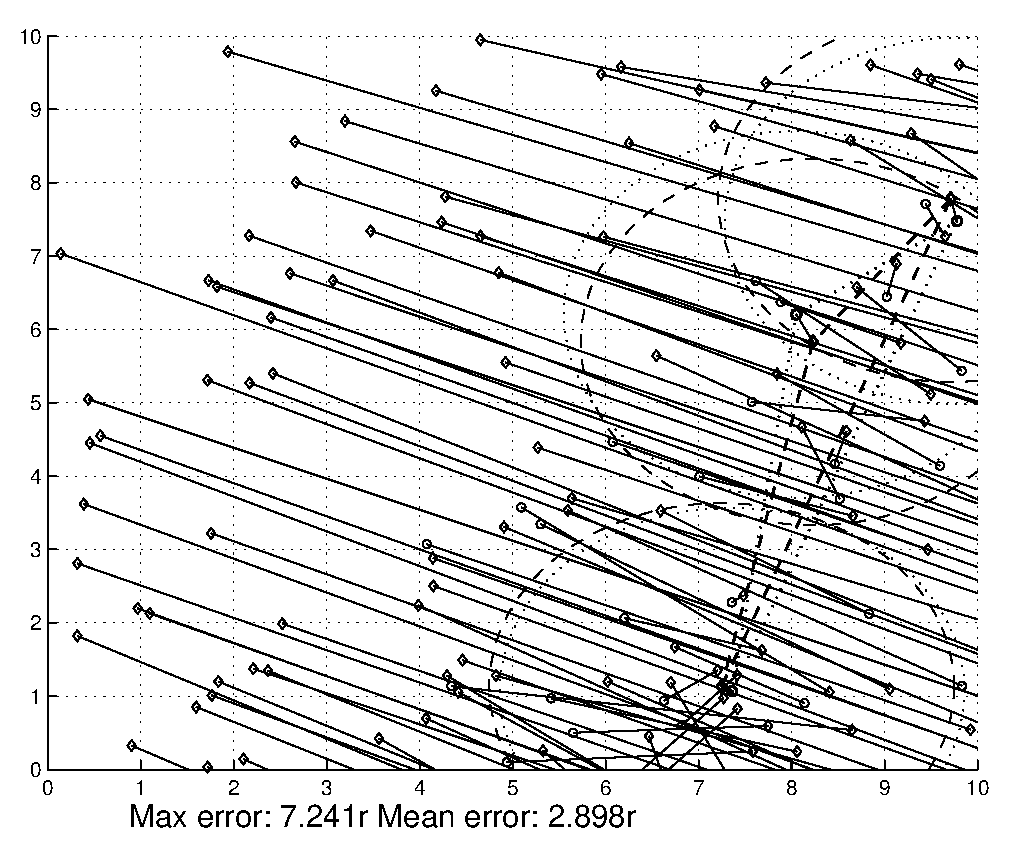
\includegraphics[width=0.5\textwidth]{outliers/AS6/AS6NetworkDiff9.eps}}
	\subfloat[A normal network difference]{\label{fig:normal1}
		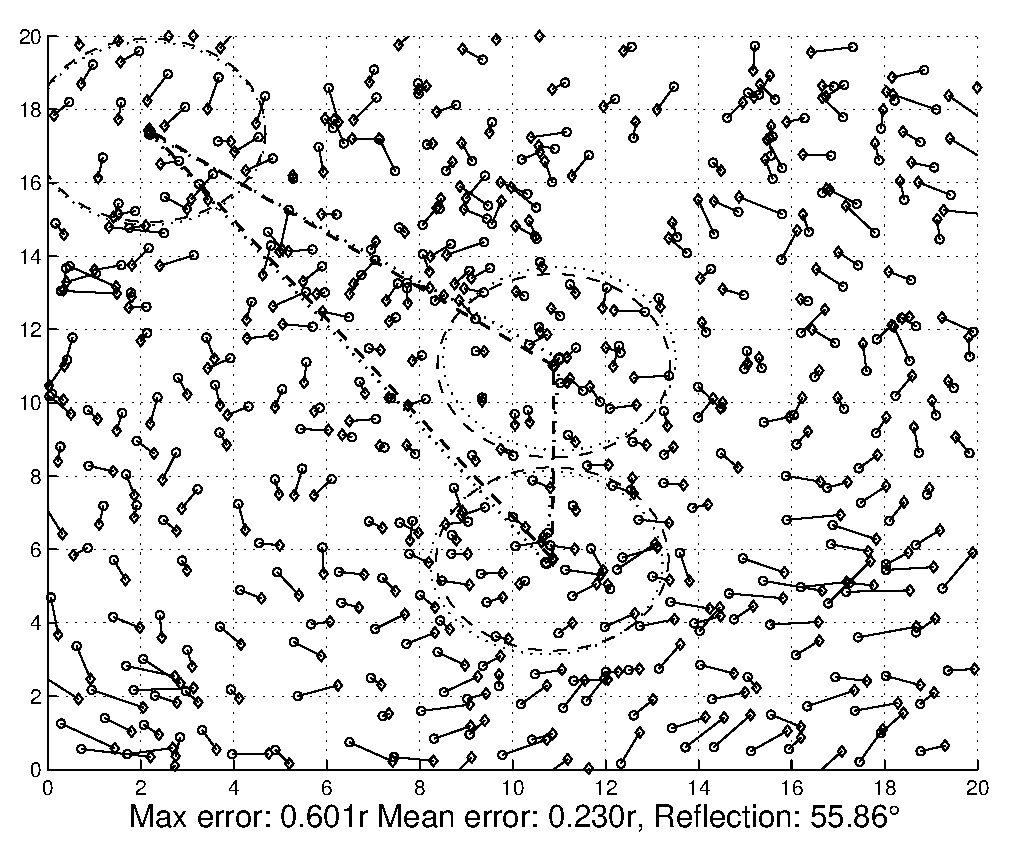
\includegraphics[width=0.5\textwidth]{outliers/normal1.eps}}		
	\label{}
	\caption{}
\end{figure}

Unfortunately, simply disabling the reflection component of the Procrustes transformation algorithm does not solve the problem.  The output of the Procrustes algorithm is a linear transformation which includes a rotation or reflection matrix.  If the determinant of that matrix is +1, then the resulting transformation has rotation.  If the determinant is -1, then the result transformation has reflection. Figure~\ref{fig:rotref} shows two different networks with 100 anchor sets each.  The figures plot the angle of rotation, as negative degrees

\begin{equation}
  \centering
	\left( \begin{array}{c} x' \\ y' \end{array}\right)~=~\left( \begin{array}{ccc} 
	cos~\theta & -sin~\theta \\ 
	sin~\theta & cos~\theta \end{array}\right)
	\left( \begin{array}{c} x \\ y \end{array}\right)
	\label{eqn:rotmatrix} 
\end{equation}
\begin{equation}
  \centering
	\left( \begin{array}{c} x' \\ y' \end{array}\right)~=~\left( \begin{array}{ccc} 
	cos~\theta & sin~\theta \\ 
	sin~\theta & -cos~\theta \end{array}\right)
	\left( \begin{array}{c} x \\ y \end{array}\right)
	\label{eqn:refmatrix} 
\end{equation}

\begin{figure}
  \centering
	\subfloat[]{\label{fig:rotref1}
		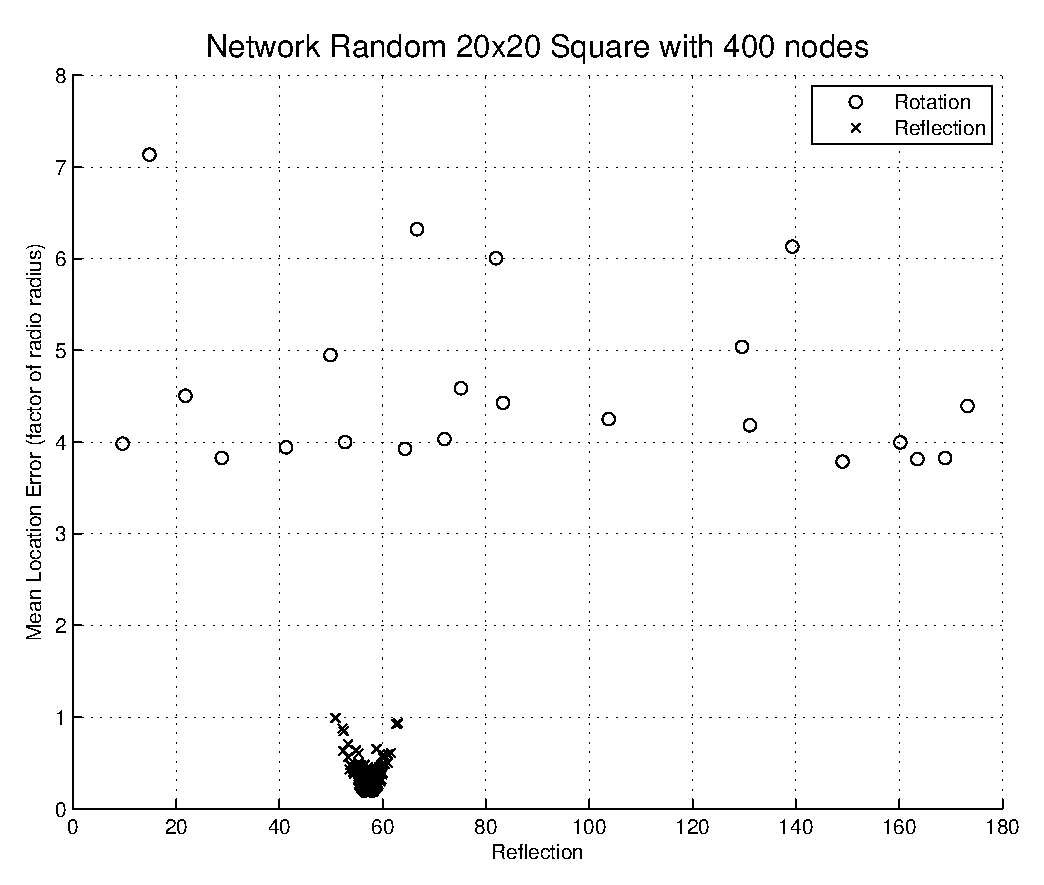
\includegraphics[width=0.5\textwidth]{rotref1.eps}}
	\subfloat[]{\label{fig:rotref2}
		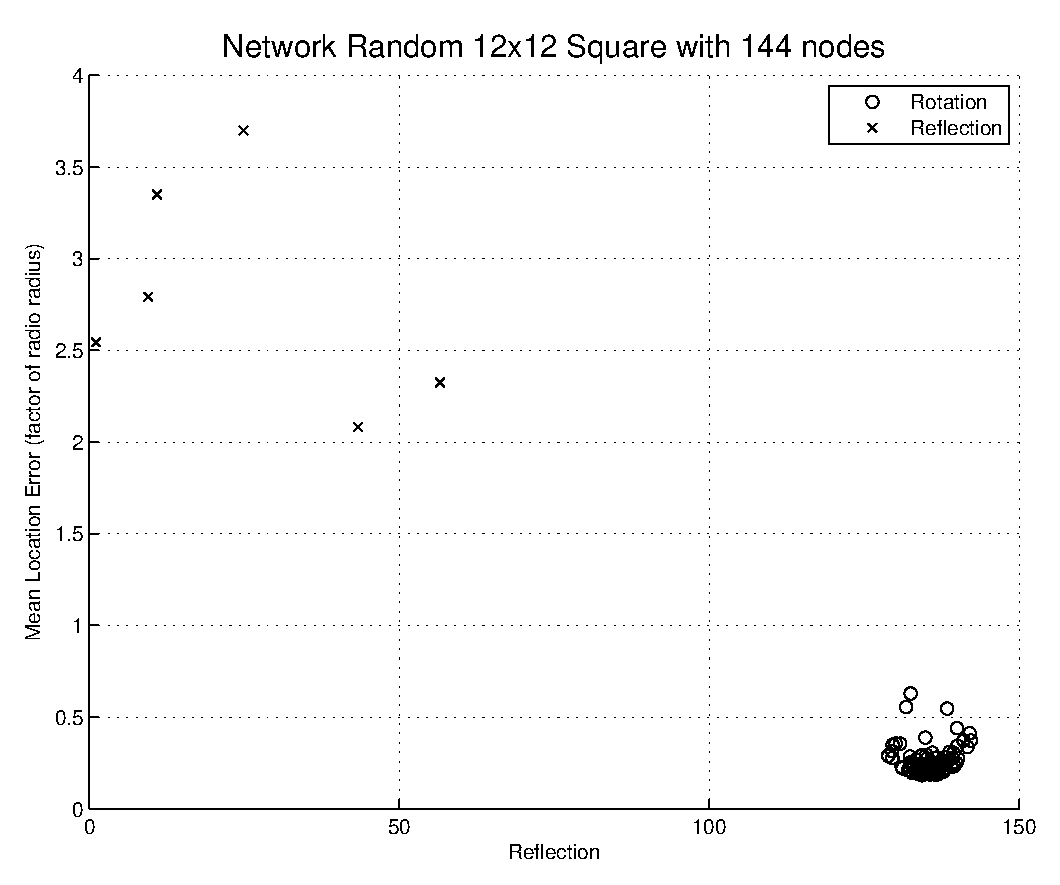
\includegraphics[width=0.5\textwidth]{rotref2.eps}}		
	\label{fig:rotref}
	\caption{Rotation and Reflection version Mean Location Error}
\end{figure}
